\documentclass[11pt]{report}

\usepackage{graphicx}
\def\d{{\rm d}}
\def\vec#1{\mbox{\boldmath $ #1$}}
\def\tens#1{\ifmmode\mathchoice{\mbox{$\sf\displaystyle#1$}}
{\mbox{$\sf\textstyle#1$}}
{\mbox{$\sf\scriptstyle#1$}}
{\mbox{$\sf\scriptscriptstyle#1$}}\else
\hbox{$\sf\textstyle#1$}\fi}



\oddsidemargin=0.1in
\topmargin=0in
\textheight=21.5cm
\textwidth=15.5cm
\parskip=1ex

%\textwidth=16cm
%\textheight=23cm
%\topmargin=-5mm
%\evensidemargin=0cm
%\oddsidemargin=0cm

 

\begin{document}
\thispagestyle{empty}
\vspace*{3cm}
\begin{center}
\Huge \bf Inversion of Stokes profiles with SIR \\
\vspace*{2cm}
\Large Luis R.\ Bellot Rubio \\
Kiepenheuer-Institut f\"ur Sonnenphysik \\
\vspace*{.5cm}
\normalsize
Version 3, 2002 March 25
\end{center}

\clearpage
\vspace*{\fill}

\hrule
\vspace*{1em}
\noindent SIR is distributed freely without any guarantee that it will work 
in your particular problem. Although you can use the code on your 
own, we STRONGLY recommend you to contact us for guidance during 
the first application of SIR to real observations.

\noindent If you find SIR useful for your work, you are kindly requested
to include the following two references in your papers:

\begin{itemize}
\item Bellot Rubio, L.R. 2003, Inversion of Stokes profiles with SIR, 
  (Freiburg: Kiepenheuer-Institut f\"ur Sonnenphysik)
\item Ruiz Cobo, B., \& del Toro Iniesta, J.C. 1992, ApJ, 398, 375 
\end{itemize}

\thispagestyle{empty}
\clearpage

\tableofcontents

\chapter{Introduction}

The present chapter gives an overview of SIR. It also describes in 
some detail the spectral synthesis calculations performed by the code 
and the inversion algorithm. The chapter contains material that
is not directly related to the use of the program. If you are not 
interested in knowing how SIR works internally, read section \ref{general}
below and skip the remainder of the chapter. If you are not familiar with
the concept of {\em nodes}, you must read section \ref{nodos} as well.


\section{General information}
\label{general}
SIR (Stokes Inversion based on Response functions) is a package for the
synthesis and inversion of spectral lines formed in the presence of
magnetic fields. The code takes into account the Zeeman-induced
polarization of the light and deals with all four Stokes parameters
($I$, $Q$, $U$, $V$) of any electric dipole transition and atomic
species. SIR was developed for the automated analysis of solar spectra
under LTE conditions.

In synthesis mode, the program calculates the Stokes
spectra\footnote{By Stokes spectra or Stokes profiles we mean the
dependence of $I$, $Q$, $U$ and $V$ on wavelength.} emerging from any
specified model atmosphere which may consist of up to two different
components (either magnetized or nonmagnetized). This is done by
solving numerically the radiative transfer equation (RTE) for polarized
light. SIR handles in a straightforward manner the particular case in
which no magnetic fields exist. Hence, it is also of interest for
integrating the scalar RTE.

In inversion mode, SIR fits any combination of observed Stokes
parameters for any arbitrary number of spectral lines. To this end, an
initial (user-provided) model atmosphere is iteratively modified until
the synthetic Stokes profiles match the observed ones. This process
yields the thermal, dynamic and magnetic structure of the atmosphere in
which the observed profiles were formed.

Spectral synthesis is carried out by means of a fast and accurate
Hermitian integration of the RTE (Bellot Rubio, Ruiz Cobo \& Collados
1998). This technique significantly improves the speed of other
well-known methods (DELO, fourth order Runge-Kutta, etc).  The 
opacity routines of Wittmann (1974) are used for the computation 
of absorption coefficients.

The inversion module of SIR implements a Marquardt nonlinear
least-squares algorithm (Press et al.\ 1986) for the minimization of
the differences between the observed and synthetic Stokes spectra.
Marquardt's method translates the nonlinear problem into a linear one, 
the solution of which is carried out by means of a modified singular 
value decomposition (SVD) algorithm (Ruiz Cobo \& del Toro
Iniesta 1992). From a mathematical point of view, the modified SVD
method implemented in SIR can be viewed as a regularization technique.
Knowledge of the partial derivatives of the Stokes parameters with
respect to the various atmospheric parameters, the so-called {\em
response functions} (RFs), is crucial for the success of the 
inversion. Thus, the synthesis module of SIR calculates all the
necessary RFs. Further details on RFs can be found in Ruiz 
Cobo \& del Toro Iniesta (1994).

The performance of SIR has been quantified by Westendorp Plaza et
al.\ (1998), who compared the behavior of SIR and the Milne-Eddington
inversion technique of Skumanich \& Lites (1992) in various numerical
experiments. SIR has been successfully applied to the study of
different solar structures observed in polarized light, such as
sunspots (Collados et al.\ 1994; Westendorp Plaza et al.\ 1997a,b,c)
and unresolved magnetic elements (Bellot Rubio et al.\ 1997), and for
non-polarized light to structures such as penumbrae (del Toro Iniesta,
Tarbell \& Ruiz Cobo 1994), solar granulation (Ruiz Cobo et al.\  1995,
1996; Rodr\'{\i}guez Hidalgo, Ruiz Cobo \& Collados 1996), and solar
oscillations (Ruiz Cobo, Rodr\'{\i}guez Hidalgo, \& Collados 1997). In
these analyses, model atmospheres were retrieved from the observed
Stokes spectra.

SIR was introduced by Ruiz Cobo \& del Toro Iniesta in 1992. Since
then, the code has been extended to make it capable of dealing with a
variety of different situations. As a result, the following programs
are now available:
\begin{itemize}
\item A code for the inversion of Stokes profiles emerging from unresolved
magnetic elements. It implements the geometry and constraints of the thin 
flux tube scenario for the analysis of active regions outside sunspots 
(Bellot Rubio, Ruiz Cobo \& Collados 1998). 
\item A code for non LTE inversion of Stokes spectra (Socas-Navarro, 
Ruiz Cobo \& Trujillo Bueno 1998).
\item MISS (Multi line Inversion of Stellar Spectra; Allende Prieto, 
Ruiz Cobo \& Garc\'{\i}a L\'opez 1998). This code is intended to fit 
observed stellar spectra, so fluxes rather than specific intensities 
are used.  
\end{itemize} 

This manual describes in detail the various algorithms behind SIR. It
also explains how to use SIR efficiently. SIR has been prepared to run
under default conditions, so previous experience is not required. For
best performance, however, the user is expected to get acquainted with
the various options allowed by the program. Although completely
automated, the inversion of Stokes spectra with SIR requires some human
intervention. Indeed, the user is expected to find the optimum
inversion conditions for the particular application of SIR at hand. This
usually requires several trial runs of the program. 


\section{The synthesis module}
\subsection{Spectral synthesis}
Spectral synthesis is carried out by solving the radiative transfer
equation for Zeeman split lines  
\begin{displaymath}
\frac{{\rm d}\vec{I}(\tau_5)}{{\rm d}\tau_5} =  \tens{K}(\tau_5) \, \left[  \vec{I}(\tau_5) 
- \vec{S}(\tau_5) \right], 
\end{displaymath}
where $\tau_5$ represents the continuum optical depth at 5000 \AA\
along the line of sight (hereafter LOS), $\tens{K}$ is the total
absorption matrix (a $4\times4$ matrix describing the absorption
properties of the atmosphere), and $\vec{S} = (S_{\scriptscriptstyle
I},S_{\scriptscriptstyle Q}, S_{\scriptscriptstyle
U},S_{\scriptscriptstyle V})^{\dag}$ the source function vector. Since
LTE conditions are assumed, the source function vector is given by
$\vec{S} = (B_\nu[T],0,0,0)^{\dag}$, with $B_\nu[T]$ the Planck's function
at the local temperature $T$. 

Except for the numerical integration of the RTE, the derivatives entering
the calculation of the RFs, and the routines for hydrostatic equilibrium, the
synthesis module of SIR is based on the code by Wittmann (1974). The
evaluation of $\tens{K}$ and $\vec{S}$ is made under the assumption of
local thermodynamic equilibrium (LTE). The atomic populations are then
computed by means of the Saha and Boltzmann equations. It is implied that
\begin{enumerate}
\item The magnetic field is strong and no quantum interferences between
Zeeman sublevels exist.

\item Collisional rates are high enough, so the various sublevels
corresponding to the same energy level are equally populated. 

\item The frequency and direction of photons scattered by an atom are
independent on the frequency and direction of the incoming photons
({\em complete redistribution on scattering}).
\end{enumerate}

The physical parameters needed to compute $\tens{K}$ are specified in
the model atmosphere, which need to be discretized in an equally
spaced logarithmic scale of the continuum optical depth at 5000 \AA\/.
At each grid point, the temperature, electron pressure,
microturbulence, magnetic field strength, azimuth and inclination of
the magnetic field vector, and LOS velocity are specified. The model
atmosphere is completed with a set of depth-independent parameters:
macroturbulent velocity, stray light contamination and filling factor
(for two component atmospheres).

The particularly simple expressions adopted by the elements of
$\tens{K}$ for Zeeman-line transfer and electric dipole transitions can
be found, e.g., in Rees (1987). Magnetooptical effects leading to
linear and circular birefringence are fully considered. The continuum
absorption coefficient $k_{\rm c}$ is evaluated for a given wavelength,
temperature and electron pressure by taking into account
contributions from H, He, H$^{-}$, He$^{-}$, H$_2^-$, H$_2^+$, C, Mg,
and Na, as well as Rayleigh scattering by H, H$_2$ and He, and Thomson
scattering by free electrons (see Wittmann 1974).  Other atomic and
molecular line opacity sources, which are neglected in the present
version of SIR, can be included in a straightforward manner.

SIR assumes hydrostatic equilibrium. After each iteration step, the 
electron pressures of the already perturbed model atmosphere are put into 
hydrostatic equilibrium by using the equation of state of
an ideal gas with variable mean molecular weight to take into account
the partial ionization of the various atomic elements. Gas pressures
are computed from temperatures and electron pressures on the
assumptions of LTE and chemical equilibrium. In this process, the
partial pressures of H, H$^+$, H$^-$, H$_2$, H$_2^+$ and other 83
elements  are determined following the strategy outlined by Mihalas
(1967). At present, the only molecules considered for the calculation
of gas pressures are H$_2$ and H$_2^+$, but up to 91 other molecules can
be included quite straightforwardly (Wittmann 1974).

The synthesis is carried out under the assumption that the predominant
broadening mechanisms are van der Waals broadening $\Gamma_6$ and
radiation broadening $\Gamma_{\rm rad}$. Stark broadening is
neglected.  Uns\"old (1955) theory is employed in the computation of
$\Gamma_6$, but the possibility of enhancing this coefficient is left
open to correct deviations of the theory (see Wittmann 1974 for
details). Thus, $\Gamma_6$ can be multiplied by a user-specified
enhancement factor $E$ that is usually in the range 1-3. SIR can handle
different enhancement factors for the different spectral lines (see 
section \ref{damping}).

Once $\tens{K}$ and $\vec{S}$ have been calculated, SIR solves the RTE
by means of an Hermitian algorithm (Bellot Rubio, Ruiz Cobo \& Collados
1998).  This new strategy was developed to accelerate the solution of
the RTE provided by the DELO method (Rees, Murphy \& Durrant 1986). The
Hermitian algorithm is based on the Taylor expansion of the Stokes vector
to fourth order in optical depth. It provides an approximation to the
evolution operator at no extra cost, which is crucial for the calculation
of response functions. The main advantages of the Hermitian method
are accuracy and speed. 

The synthesis module of SIR is capable of dealing with blends. It is
possible, for example, to synthesize the Stokes profiles of a
particular spectral line by including the contribution of nearby
lines.  This is achieved by adding, at every wavelength, the absorption
matrices of the different contributing atomic transitions. 

The various steps through which SIR calculates simulated Stokes spectra 
are:

\begin{enumerate}
\item The files containing the model atmosphere and the atomic parameters 
of the lines to be synthesized are read. 
\item The RTE is integrated numerically for the wavelengths specified
in a wavelength grid file. If the atmosphere consists of two
different components, the Stokes spectra emerging from each component,
$\vec{I}_1(\lambda)$ and $\vec{I}_2(\lambda)$, are computed
individually and then mixed according to their filling factors
$f_1$ and $f_2$, with $f_1 + f_2=1$. In this case, the emergent Stokes 
spectrum is
\begin{displaymath}
\vec{I} = f_1 \, \vec{I}_1 + f_2 \, \vec{I}_2,
\end{displaymath}
\item The same height-independent macroturbulent velocity $v_{\rm mac}$ 
is assumed for all spectral lines. The effect of the macroturbulence is 
simulated by convolving $\vec{I}$ with a gaussian 
\begin{displaymath}
M(\lambda - \lambda_0, v_{\rm mac}) = \frac{1}{\sqrt{2\pi} \; \sigma} 
{\rm e}^{{-\frac{(\lambda-\lambda_0)^2}{2\sigma^2}}},
\end{displaymath}
where $\sigma \equiv \lambda_0 v_{\rm mac}/c$, $\lambda_0$ is the central
wavelength of the transition and $c$ is the speed of light. Additionally, 
the macroturbulent-broadened profiles ($\vec{I}^* = \vec{I}*M$) may be 
convolved with the PSF of the spectrograph if it is available. 
\item The last step in simulating the observed profiles $\vec{I}_{\rm obs}$ 
is to add a user-provided stray light spectrum $\vec{I}_{\rm str}$ that 
contributes a fraction $\alpha$ to $\vec{I}_{\rm obs}$:
\begin{displaymath}
\vec{I}_{\rm obs} = (1-\alpha) \, \vec{I^*} + \alpha \vec{I}_{\rm str}.
\end{displaymath}
\end{enumerate}

\subsection{Response functions}
Response functions (RFs) to the various atmospheric parameters $x(\tau)$,
$\vec R_x (\lambda, \tau)$, are calculated at every optical depth and
wavelength according to the formula
\begin{displaymath}
   \vec R_x (\tau) = \tens{O}(0, \tau)
   \left\{ \tens{K}(\tau) \frac {\partial \vec{S}(\tau)} {\partial x} -
   \frac {\partial \tens{K}(\tau)} {\partial x}
   \left[ \vec{I}(\tau) - \vec{S}(\tau) \right ] \right\} ,
\end{displaymath}
where $\tens{O}(0,\tau)$ represents the evolution operator from $\tau$
to the surface. By definition, the modification of the emergent Stokes
spectrum $\delta \vec{I}(\lambda)$ after perturbations $\delta x(\tau)$
of the atmospheric parameter $x$ at optical depth $\tau$ is given by
\begin{equation}
\label{defrf}
\delta \vec{I}(\lambda) = \int_0^{\infty} \vec{R}_x (\lambda, \tau) \, \delta x(\tau) \, {\rm d}\tau.
\end{equation} 

If a nonzero macroturbulence is used to synthesize the emergent Stokes
spectrum, all the RFs have to be convolved with $M$ as well. The same
applies if the spectrograph profile is taken into account.

\section{The inversion module}
\label{nodos}
The inversion of Stokes profiles proceeds by minimizing a merit function which 
is the sum of the squared differences between observed and synthetic data 
weighted by the uncertainties of the observations and by some factors 
$w_{ki}^2$. The merit function is defined as
\begin{equation}
\label{chi}
\chi^2 \equiv \frac{1}{\nu} \sum_{k=1}^4  \sum_{i=1}^M  
\left[ I_k^{\rm obs}(\lambda_i) - I_k^{\rm syn}(\lambda_i) \right]^2 \, 
\frac{w_{ki}^2}{\sigma_{ki}^2},
\end{equation}
where index $k=1,\ldots,4$ samples the 4-component vectors containing
the observed (obs) and synthetic (syn) Stokes profiles, $i =
1,\ldots,M$ sample the wavelengths at which the spectrum has been
measured, $\nu$ is the number of degrees of freedom (i.e., the number
of observables minus the number of parameters to be inverted) and
$\sigma_{ki}$ are the uncertainties of the observations. SIR
automatically adjusts the factors $w_{ki}^2$ so as to give the same
relative weight to the Stokes parameters of different spectral lines,
independently of their amplitudes. The user may specify that more weight is to be 
assigned to a particular Stokes parameter. For example, more weight
could be desired for Stokes $V$ when analyzing magnetic regions.
Subsection \ref{profiles} explains in detail how to vary the relative weights
of the various Stokes parameters. By default, SIR assumes that the
uncertainties $\sigma_{ki}$ are all equal to a constant value
$\sigma$ given by the signal-to-noise ratio of the observations.  
However, $\sigma_{ki}$ is set to $10^{15}$ for points in the 
observed profiles that will {\bf not} be considered for inversion. This
option is useful, for example, when the intensity profiles are
contaminated by blends of solar or terrestrial origin, but the
corresponding polarization profiles ($Q$, $U$ and $V$) are not. In this
case, one may invert the whole $Q$, $U$ and $V$ profiles and the portion
of the intensity profile that is not contaminated with blends by simply 
replacing the undesired intensities by $-1.0$ in the file containing the 
observed spectrum (see Section \ref{profiles} for more details). When SIR finds 
values smaller than $-1.0$ for any of the Stokes parameters, the 
corresponding $\sigma_{ki}$ are set to $10^{15}$, the consequence 
being that such data points are not taken into account in the fit.  


\begin{figure}[tb]
		\centering
		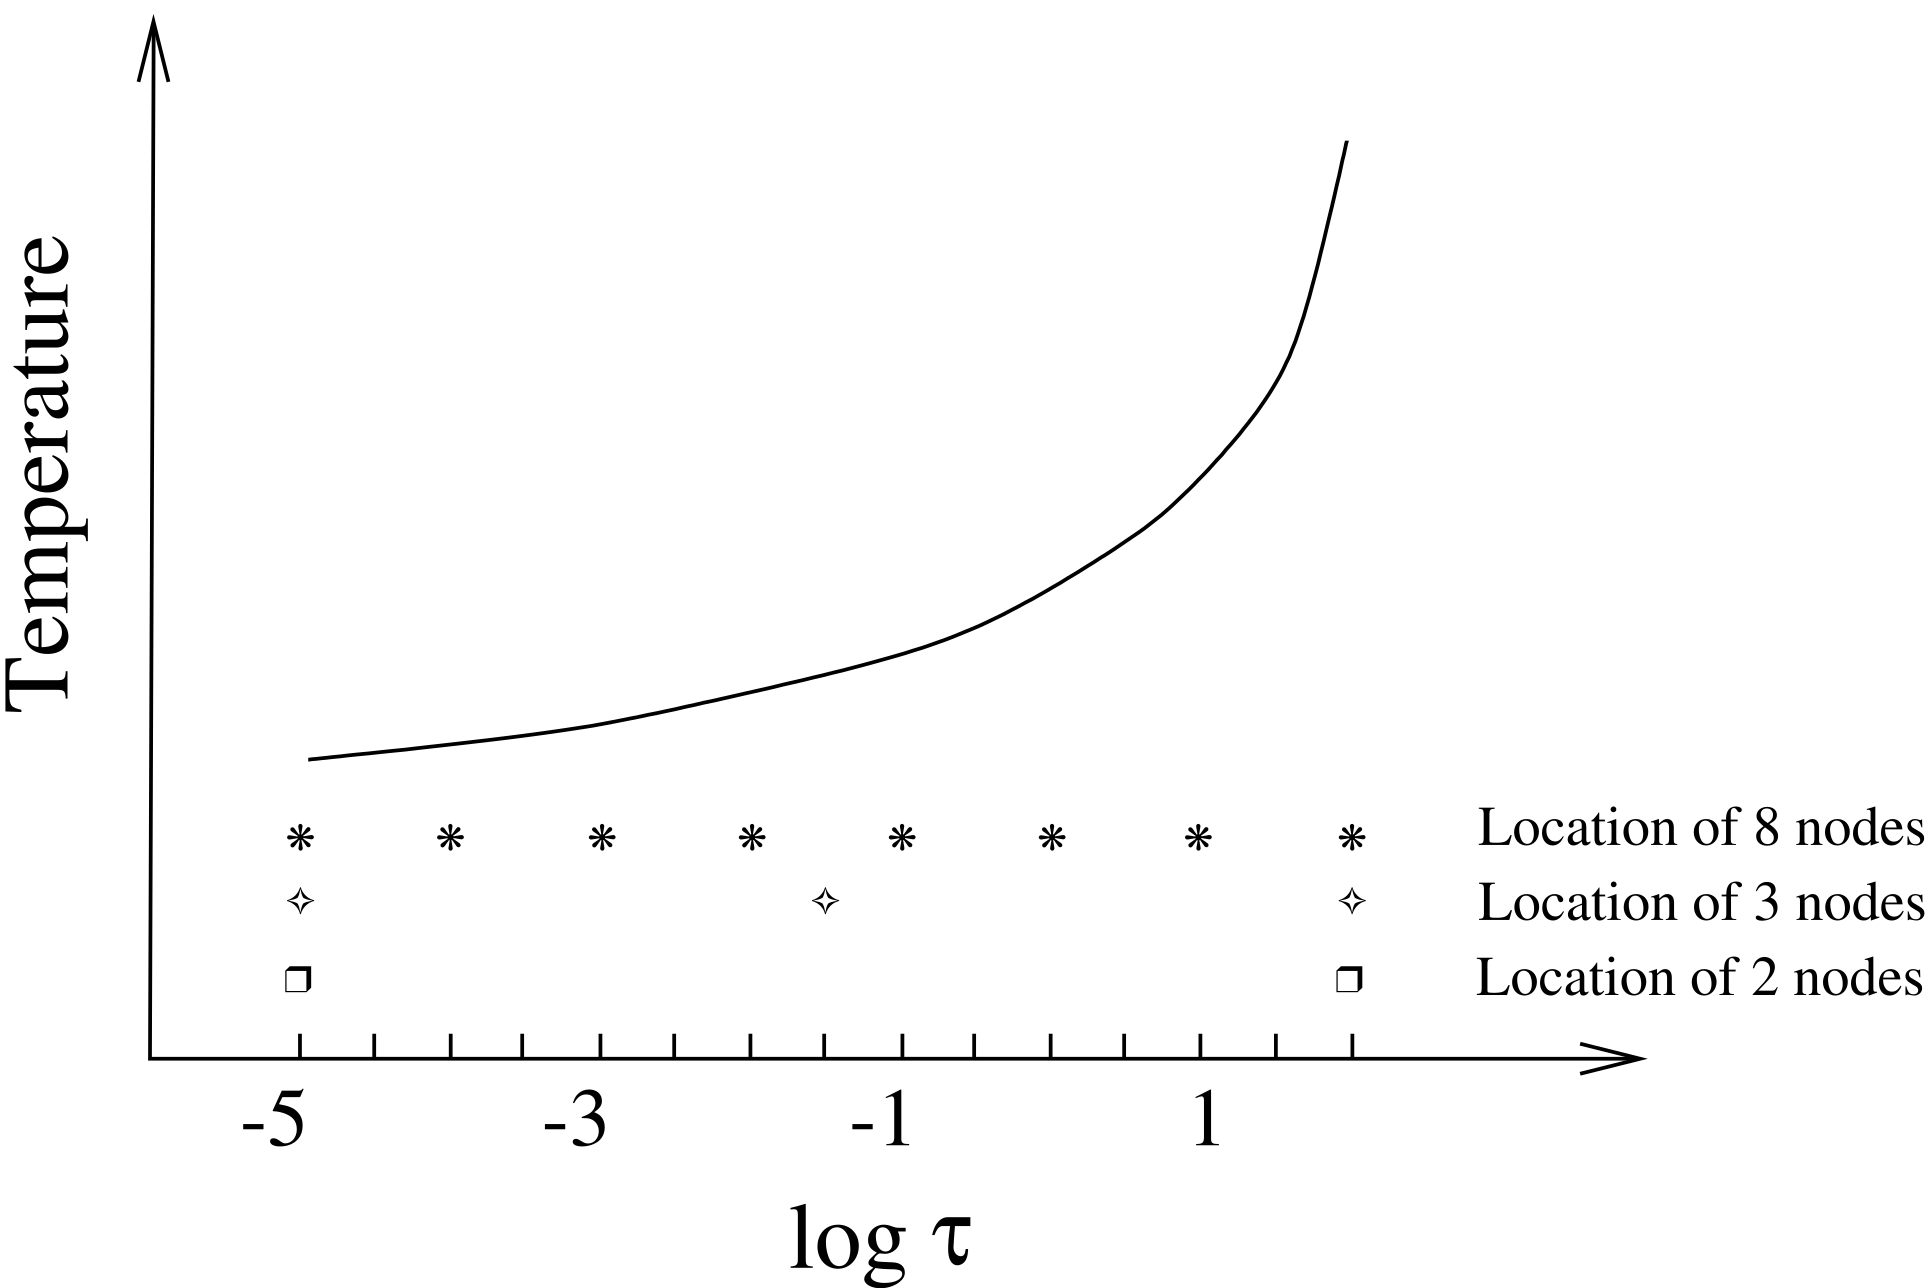
\includegraphics[width=10cm]{nodos.png}
		\caption{Schematic explanation of how the nodes are chosen. The
particular case of temperature ($T$) is considered. The atmosphere is
discretized in the logarithmically evenly spaced grid shown in the
$x$--axis, the step size being $\Delta {\rm log} \tau = 0.5$ in this
particular example. The optical depths at which perturbations of the
temperature will be sought are determined by the number of nodes
selected.  If the user specifies two nodes, perturbations of $T$ at
$\log \tau = -5.0$ and $\log \tau = 2.0$ will be found. With three
nodes, perturbations will be found at $\log \tau = -5.0$, $\log \tau =
-1.5$ and $\log \tau = 2.0$. The same scheme applies with a larger
number of nodes.  Note that five nodes cannot be used here because
there are no sufficient spatial points in the grid to produce an even
distribution of the nodes through the whole atmosphere.}
 \label{nodosfig}

\end{figure}


The minimization of Eq.\ (\ref{chi}) is carried out iteratively by
modifying an initial user-provided model atmosphere. This process
yields the perturbations of the guess atmosphere required for the
synthetic spectrum to match the observed one. However, the minimization
of $\chi^2$ is complex because $\vec{I}^{\rm syn}$ depends nonlinearly
on the various atmospheric parameters. To handle this problem, SIR
implements a Marquardt algorithm (Press et al.\ 1986).  Marquardt makes
use of the derivatives of $\chi^2$ with respect to the model
parameters. It turns out that these derivatives can be expressed in
terms of RFs (Ruiz Cobo \& del Toro Iniesta 1992), which explains the
relevance of the RFs for the inversion.

In order to reduce the number of free parameters, the perturbations of
the depth-dependent physical quantities characterizing the initial guess 
model atmosphere are calculated only for a few grid points (called {\em nodes}) of the
spatial grid in which the atmosphere is discretized. For each physical
quantity (e.g., temperature, LOS velocity, etc), the atmosphere is
represented by a different set of nodes. The perturbations of the
various parameters in all the remaining grid points are approximated 
by linear or cubic-spline interpolation of the perturbations at the nodes.  


Figure \ref{nodosfig} explains in more detail the concept of nodes
introduced by SIR. Once the number of nodes has been specified for a
given physical quantity, the code locates the optical depths at which
perturbations will be sought. If only one node is allowed, the
perturbation suggested by Marquardt is added to the values of the
physical quantity under consideration at all heights (i.e., its depth
stratification is modified by a constant perturbation). With two nodes, the
perturbations at the nodes are interpolated linearly to the whole
atmosphere.  With three nodes, either linear or parabolic interpolation 
is used. With four or more nodes, linear or cubic-spline interpolation 
is applied. Sect.\ 3.2 explains how to select one or other type of
interpolation.

SIR allows the user to specify the number of nodes for each physical
quantity. Note that the number of free parameters equals the sum of the
number of nodes adopted for the various physical quantities. The set of
iterations carried out without modifying the number of nodes is called a
{\em cycle}. Usually, SIR needs two or three cycles to arrive at the final
solution. In each iteration cycle, the number of free parameters is normally 
increased to permit more flexibility to the solution.

\subsection{Error estimation}
For the computation of errors in the retrieved parameters we 
follow a simple physical argument. According to Eq.\ (\ref{chi}), the weighted 
squared difference between the observed and synthetic spectra 
can be written as 
\begin{equation}
\sum_{i,k} \delta I^2_{ki} \frac{w^2_{ki}}{\sigma_i^2} = \nu \chi^2,
\end{equation}
with $\delta I_{ki} \equiv I^{\rm obs}_k(\lambda_i) - 
I^{\rm syn}_k(\lambda_i)$. Now assume that $m$ model parameters 
are to be inverted, each one being responsible of a fractional part 
$1/m$ of the observed differences $\delta I^2_{ki}$. With these hypotheses 
we can find a set of perturbations $\delta x(\tau)$ to the original parameters 
that minimize $\chi^2$. Using the definition of the RFs (see Eq.\ \ref{defrf}) 
we have 
\begin{equation}
\frac{\delta I_{ki}}{\sqrt{m}}  = R_{x,k}(\lambda_i,\tau) \delta x(\tau) 
\Delta \tau,
\end{equation}
and so
\begin{equation}
\label{error}
\sigma^2_{x(\tau)} \equiv [\delta x(\tau)]^2 = \frac{\nu \chi^2}{m (\Delta \tau)^2 \;
\sum_{i,k} R^2_{x,k}(\lambda_i,\tau) \; w^2_{ki}/\sigma^2_i}.
\end{equation}
We have implicitly assumed that all model parameters are independent, so
changes in a given parameter do not influence the remaining ones. Indeed, 
Monte Carlo simulations have demonstrated that the actual uncertainties 
are well represented by Eq.\ (\ref{error}).  As it might have been 
expected, uncertainties $\sigma_{x(\tau)}$ are proportional to the inverse 
of the RF to changes in $x(\tau)$. Therefore, parameters that have little 
influence on the emergent Stokes spectrum show the largest uncertainties. 
This is the case for most parameters outside the region where the 
spectral lines used are formed.


\chapter{Installing and running SIR}
This chapter provides a brief guide for getting and installing SIR. To
date, the program has been run successfully in Sun and Alpha
workstations. More platforms are expected to be added to the list in
the near future. 

\section{Where to get the program}
For IAC users, the latest version of SIR is in the directory
\begin{center}
{\tt /net/camello/scratch1/choco\_luis/lbellot/lbellot/sir/latest},
\end{center}
where you will find the {\tt sir.tar} file. This file contains the following 
directories: 
\begin{itemize}
\item {\tt default}. This subdirectory keeps default files. 
\item {\tt idl}. Several IDL procedures for visualizing model atmospheres
and Stokes profiles. There are also some utilities for extracting observed
profiles from the IDL FTS spectral atlas.
\item {\tt manual}. This subdirectory contains the present manual.
\item {\tt models}. Here you will find some standard model atmospheres
which may be of use in real inversions. A number of utilities for modifying
these models or others are provided as well.
\item {\tt program}. This subdirectory keeps the source programs and the
macros needed to compile SIR.
\item {\tt test}. This subdirectory contains a particular inversion intended
to test the degree of success of the installation. 
\end{itemize}

You may also obtain the {\tt sir.tar} file by sending an email to
{\tt lbellot@kis.uni-freiburg.de}. In the near future we intend to make SIR available
through ftp, but this is not implemented yet.

\section{How to install the program}
To install the program, create a directory called {\tt sir} in your home
directory, copy the {\tt sir.tar} file to that directory and type
\begin{flushleft}
{\tt tar xvf sir.tar}
\end{flushleft}
The files will be extracted with their original path names. This will
create the directories mentioned above.

Now you have to compile and link the various subroutines. To this end,
move to the directory {\tt $\sim$/sir/program}. There you will find
three Unix (cshell) scripts which will do the job:
\begin{itemize}
\item {\tt compile}. This script invokes the Fortran 77 compiler. It
compiles {\em one} single routine and updates the resulting object file in 
the SIR library ({\tt libreria.a}). The macro is invoked by typing
{\tt compile name\_of\_routine} (without the .f extension).
\item {\tt compileall}. This script compiles all routines. No arguments
are needed.
\item {\tt linkprog}. This script links the {\tt sir.f} main program and
the SIR library. After having compiled all routines with 
{\tt compileall}, you must type {\tt linkprog sir}. 
\end{itemize}
There are different macros for the different platforms. For Sun Sparc 
workstations, HP workstations, and Pentium-based machines, use the
scripts ending in {\tt \_sun}, {\tt \_hp}, and {\tt \_linux}, respectively.

Once the commands {\tt compileall} and {\tt linkprog sir} have been
issued, the executable file is available under the name {\tt sir.x}. 

\section{Optimizing SIR at installation time} 
SIR has been prepared to minimize the CPU and memory usage of the
machine. If you want to take advantage of this capability when dealing 
with a particular problem, you should (re)compile all the routines 
to specify the appropriate array dimensions to be used for the particular 
application of SIR at hand.   

In the {\tt $\sim$/sir/program} directory there is a file called 
{\tt PARAMETER} which provides the values of the following 
parameters at compilation time:
\begin{itemize}
\item {\tt kt}: Maximum number of spatial points in the grid used to discretize
the model atmosphere. 
\item {\tt kn}: Maximum number of nodes allowed for each of the depth-dependent
physical quantities. By definition, {\tt kn}~$\leq$~{\tt kt}. 
\item {\tt kl}: Number of spectral lines (including blends) to be inverted.
\item {\tt kld}: Total number of wavelength samples.
\end{itemize}
At installation, the {\tt PARAMETER} file provides the following
default values:  ${\tt kt} =64$, ${\tt kn} = 64$, ${\tt kl}=100$ and
${\tt kld} = 600$. Note that, whenever you change any of these
array dimensions, the whole set of routines must be compiled again 
(with {\tt compileall}) and linked (with {\tt linkprog sir}).

\section{Running SIR}
Once SIR has been properly installed, it can be run by typing either 
\begin{flushleft}
{\tt sir.x}
\end{flushleft}
 or 
\begin{flushleft}
{\tt echo sir.trol | sir.x} 
\end{flushleft} 
The second form is used to directly provide the code with the name of
the control file ({\tt sir.trol}, in this example). If the first
command is issued, the program will ask for the name of the control
file right after having been called up. In order to run SIR without
having to specify where the {\tt sir.x} program resides, it is
advisable that the directory {\tt $\sim$/sir/program} be included in the
user's path. This can be done by adding the following sentences to the
{\tt .cshrc} file in the home directory
\begin{flushleft}
\tt
set SIRpath    = ( $\sim$/sir/program/ ) \\
set path    = (\$path \$SIRpath)
\end{flushleft}

At present, SIR inverts one single set of Stokes spectra per program 
call. If time series or two-dimensional maps of Stokes spectra are to 
be analyzed, the user may write very simple Unix scripts to run SIR 
repeatedly without having to invoke the program for each of the 
individual spectra. An example of such an script will be given 
in Section \ref{corremuchos}.

\section{Checking the installation}
The {\tt $\sim$/sir/test} directory contains the results of a particular
inversion which may be used to test the behavior of the code in other
machines. To this end, run SIR from that directory by typing {\tt 
echo sir.trol | sir.x} and compare the temperatures in the resulting 
model atmospheres (called {\tt guess\_1.mod}, {\tt guess\_2.mod} and 
{\tt guess\_3.mod}) with those in the test model atmospheres 
{\tt test\_1.mod}, {\tt test\_2.mod} and {\tt test\_3.mod}. 

If everything is correct, the differences between the temperatures
in the test models and the model atmospheres resulting from the
inversion should be small (differences of up to 200-500 K may be
present in the very deep and upper layers; such differences are
absolutely normal). If this is not the case, the models will differ 
significantly, revealing that the compiler does not behave as 
expected. Should this occur, please contact 
lbellot@kis.uni-freiburg.de or brc@iac.es.  

Normally, malfunctioning of the code is produced by the way the
compiler handles local variables upon re-entering a given subroutine.
SIR was developed using a compiler that does {\em not} initialize to
zero the local variables whenever a subroutine is reentered (i.e., the
variables from the previous call are kept), but other compilers do,
causing the program to crash.



\chapter{Fundamentals of operation}
In the following, the various input/output files used by SIR are 
described in detail. Some useful hints are also given.  

\section{Introduction}
Major efforts have been made to ensure that SIR will detect and report
the errors caused by improper use of established formats and/or typos
in the input files. In addition, we have tried to make SIR as
user-friendly as possible, in the sense that the human interaction with
the program has been reduced to a minimum.  However, SIR cannot be
regarded as a black box that once fed with the observations will
produce good results. Indeed, some (crucial) intervention is
expected from the user, namely the selection of the optimum number of
nodes. Although the program has been provided with automatic procedures
for selecting nodes, these are reserved for the inexperienced user. The
success of the inversion critically depends on the experience of the
user, so playing with the code is highly recommended before inverting
real observations. We also advise you to contact us for guidance during 
the first applications. Our feedback will be important for you to be 
sure that SIR is being used in the proper way.  

SIR receives information via the input files described in this chapter.
At present, to change the conditions under which the inversion is
carried out, the user has to edit these files by hand and stick to the
rules given below to prevent errors from occurring. Work is currently
being done to develop a window interface to SIR which will be
used to control the various options without having to modify any file
by hand.    

\section{The control file}
SIR uses the files and performs the operations specified in the 
control file. Control files are recognized by the extension {\tt .trol}. 
 
\begin{table}
\small
\tabcolsep 0.1em
\caption{Example of a control file \protect \\ 
         }
\label{control}
\begin{tabular}{lrcll}
 &  & &            &       \\
 &  & &            &       \\

Number of cycles          &(*)&:&3             &! (0=synthesis)  \\
Observed profiles         &(*)&:&profiles.per &             \\
Stray light file          &   &:&stray.per    & ! (none=no stray light contam)\\
PSF file                  &   &:&psf.dat      & ! (none=no convolution with PSF)\\
Wavelength grid file      &(s)&:&grid.grid     & ! (none=automatic selection)\\
Atomic parameter file      &  &:&LINEAS       & ! (none=DEFAULT LINES file)\\
Abundance file           &   &:&THEVENIN  \phantom{ho}   & ! (none=DEFAULT ABUNDANCES file)\\
Initial guess model 1     &(*)&:&guess1.mod   &\\
Initial guess model 2     &   &:&guess2.mod   &\\
Weight for Stokes I        &  &:1 &            &! (DEFAULT=1; 0=not inverted)\\
Weight for Stokes Q        &  &:1 &            &! (DEFAULT=1; 0=not inverted)\\
Weight for Stokes U        &  &:1 &            &! (DEFAULT=1; 0=not inverted)\\
Weight for Stokes V        &  &:10 &            &! (DEFAULT=1; 0=not inverted)\\
AUTOMATIC SELECT. OF NODES?&  &: &            &! (DEFAULT=0=no; 1=yes)\\
Nodes for temperature 1    &  &:&1,5,10,12       &        \\
Nodes for electr. press. 1 &  &:&             &        \\
Nodes for microturb. 1     &  &:&0,1            &       \\
Nodes for magnetic field 1 &  &:&1		   &\\
Nodes for LOS velocity 1   &  &:&     &         \\
Nodes for gamma 1          &  &:&     &          \\
Nodes for phi 1            &  &:&     &          \\
Invert macroturbulence 1?  &  &:&1    &        ! (0 or blank=no, 1=yes)\\
Nodes for temperature 2    &  &:&     &          \\
Nodes for electr. press. 2 &  &:&     &                \\
Nodes for microturb. 2     &  &:&     &              \\
Nodes for magnetic field 2 &  &:&     &\\
Nodes for LOS velocity 2   &  &:&     &         \\
Nodes for gamma 2          &  &:&     &          \\
Nodes for phi 2            &  &:&     &          \\
Invert macroturbulence 2?  &  &:&     &        ! (0 or blank=no, 1=yes)\\
Invert filling factor?     &  &:&     &        ! (0 or blank=no, 1=yes)\\
Invert stray light factor? &  &:&1    &        ! (0 or blank=no, 1=yes)\\
mu=cos (theta)              & &:&     &        ! (DEFAULT: mu=1.)\\
Estimated S/N for I         & &:&200  &        ! (DEFAULT: 1000) \\
Continuum contrast          & &:&     &        ! (DEFAULT: not used)\\
Tolerance for SVD           & &:&     &        ! (DEFAULT value: 1e-4)\\
Initial diagonal element    & &:&     &        ! (DEFAULT value: 1.e-3) \\
Splines/Linear Interpolation& &:&     &        ! (0 or blank=splines, 1=linear) \\
Gas pressure at surface 1   & &:&     &        ! (0 or blank=Pe boundary cond.) \\
Gas pressure at surface 2   & &:&     &        ! (0 or blank=Pe boundary cond.) \\
Magnetic pressure term?     & &:&     &        ! (0 or blank=no, 1=yes) \\
NLTE Departures filename    & &:&     &        ! blank= LTE (Ej. depart\_6494.dat') \\
\end{tabular}
\end{table}

Control files have 42 lines that must be ordered as in the example of
Table \ref{control}. Each line is divided in three parts. The first one
extends until the colon mark (:). The second extends from the colon to
the exclamation mark (!). The third one goes from the exclamation mark
to the end of the line. These three parts contain the name of the field, the
information to be used by SIR, and comments or additional explanations
for the user, respectively. SIR ignores all what is written in the line 
after the exclamation mark.

The first line in the control file specifies the number of cycles of
the inversion (i.e., how many times the number of nodes is going to
change). The following eight lines provide SIR with the names of 
several input files. Full paths (up to 300 characters) can be used
here. The remaining lines specify details of the inversion.

The information required by SIR is contained in the second part of each
line. More than one file name or numerical value can appear there, {\em
always separated by commas}. At the beginning of each iteration cycle,
SIR will read the appropriate name or number in the sequence. For
example, the sequence {\tt 1,5,10,12} in the field {\tt Nodes for
temperature 1} in Table \ref{control} instructs SIR to use one node for
the first cycle, 5 nodes for the second, and 10 nodes for the third
cycle. Note that only three cycles will be performed (as specified in
the first line of the file), so the last number in the sequence (12) is
not used. In much the same way, {\em every} line of the control file
may contain different variables to be used in the corresponding
iteration cycle.

Many lines in the control file may be left blank, in which case SIR
will adopt {\em default} values for the relevant parameters. Other lines,
however, need to be filled with the appropriate information. For
convenience, these lines are marked with an asterisk (*) before the
colon. In synthesis mode, providing the information for lines marked
with (s) before the colon is {\bf mandatory}.

Taking the control file of Table \ref{control} as an example, we now
briefly discuss the exact meaning of the different entries:
\begin{itemize}
\item {\tt Number of cycles}. Compulsory. This parameter indicates the
number of iteration cycles to be carried out. In our example, SIR is
forced to perform three cycles. For synthesis of Stokes spectra
(without inversion), the number of cycles should be set to zero. 
If the number of cycles is $-1$, response functions will be computed and
saved to disk.
\item {\tt Observed profiles}. Compulsory. This is the name of the file
containing the observed profiles (in inversion mode) or the name of the
file where the synthesized profiles will be stored (in synthesis mode).
\item {\tt Stray light file}. Name of the file containing the stray
light intensity profile ($\vec{I}_{\rm str}$). If no name is specified,
the synthetic profiles will be computed with $\alpha=0$ (i.e., no stray
light contamination). The wavelengths of the stray light profile
must coincide with those in the observed profiles, otherwise
an error message will be issued and the program will abort.
\item {\tt PSF file}. Name of the file containing the spectrograph profile. If
no name is specified, the synthetic profiles are not convolved with the PSF of
the spectrograph.
\item {\tt Wavelength grid file}. Compulsory in synthesis mode, optional otherwise. 
This is the name of the file specifying the wavelengths at which the profiles are
known. In inversion mode, the wavelengths can be read from the profiles themselves,
so there is no need to specify any wavelength grid. However, this file must be
used when blended lines are desired (see below). 
\item {\tt Atomic parameter file}. Name of the file containing the atomic data
for the spectral lines considered. If no name is specified, SIR will look for
the default {\tt LINES} file in the {\tt $\sim$/sir/default/} directory.
\item {\tt Abundance file}. Name of the file containing the abundances of the
various chemical species in the solar atmosphere. If no name is specified, the
default {\tt ABUNDANCES} file in the {\tt $\sim $/sir/default} directory will be used. 
We normally use the THEVENIN abundance file.

\item {\tt Initial guess model 1}. Compulsory. This is the name of the model
atmosphere to be used for synthesis (if in synthesis mode) or the name of 
the initial guess model (if in inversion mode). The format of this file is
explained in Section \ref{modelo}. In our example, the starting model
is called {\tt guess1.mod}. The improved model resulting from the first iteration
cycle will be called {\tt guess1\_1.mod}, and will be read as the initial guess model
for the second iteration cycle. After this new cycle, the improved model is
{\tt guess1\_2.mod}, and so on. An inversion run may be started with an initial
guess model called {\tt model\_4.mod}, for instance. In this case, SIR will take
care of updating the subindex whenever an iteration cycle has finished. Thus, the
improved model resulting from the first cycle will be called {\tt model\_5.mod}. 

\item {\tt Initial guess model 2}. Same as above, but only if a two-component 
model atmosphere is being used. The name of the initial guess model for the second
component does not need to coincide with that of the first component. Thus, 
for instance, one might start the inversion with an initial second component
called {\tt model2\_7.mod}. The number of depth points in model 2 must coincide
with that in model 1. Otherwise, the program is aborted.

\item {\tt Weights for Stokes I, Q, U and V}. These parameters indicate
the relative weight of Stokes $I$, $Q$, $U$ and $V$ in the $\chi^2$
merit function. In the example of Table \ref{control}, Stokes $V$ is
given ten times more weight than Stokes $I$, $Q$ and $U$. If no weight
is specified, a default weight equal to unity will be assigned. Zero
weights imply that the corresponding Stokes parameters will not be
inverted.

\item {\tt AUTOMATIC SELECT. OF NODES?} If this parameter is set to
zero (the default), the user must specify by hand the number of nodes
to be used for each physical quantity in all the iteration cycles. If this
parameter is set to one, then a simple pattern for the automatic
selection of nodes is adopted. Such a pattern takes advantage of the
fact that the Stokes profiles are most sensitive to temperature, while
the other physical quantities are less important to first order. Then,
the temperature is given more flexibility (ie., more nodes) right from
the very beginning. To this end, the divisors of ${\tt ntau} - 1$
(where {\tt ntau} is the number of grid points in the discretized
atmospheres) are found. Let us denote the $i$th divisor (from the
smallest to the largest one) by $d(i)$.

The automatic sequence of nodes for temperature would be: $d(3)$,
$d(4)$, $d(5)$, and so on. Thus, for the $j$th cycle, the number of
nodes assigned to temperature would be $d(j+2)$. For the other
depth-dependent physical quantities, the number of nodes assigned 
at cycle $j$th is $d(j)$.

Even if automatic selection of nodes is in effect, the user can decide
which parameters are to be determined. Imagine, for instance, that the
temperature of model 1 is to be improved right from the first cycle,
while the temperature of the second component is desired to improve
only after the first cycle. If automatic selection of nodes has been
allowed, then the user should write {\tt 1} in the field {\tt Nodes for
temperature 1}, and {\tt 0,1} (or {\tt 0,3}, for example) in the field
{\tt Nodes for temperature 2}. The zero in the second field instructs
SIR not to invert the temperature of model 2 in the first cycle. The
numbers one or three (no matter the value of this number provided it is
not zero) indicates that the temperature of the second component will
be modified already in the second cycle (with the number of nodes being
determined automatically).

\item {\tt Nodes for the various atmospheric parameters in models 1 and 2}. The
following eighteen fields specify the number of nodes to be 
used in each iteration cycle (only if manual selection of nodes has
been chosen). Consider the following example from our control file in
Table \ref{control}:
\begin{flushleft}
\tt 
\tabcolsep 0.1em
\begin{tabular}{lcl}
Nodes for temperature 1    &:&1,5,10,12         \\
Nodes for electron pressure 1 &:&                  \\
Nodes for microturbulence 1     &:&0,1               \\
Nodes for magnetic field 1 &:&1	
\end{tabular}
\end{flushleft}
In the first cycle, temperature will be given one node, microturbulence
zero nodes, and magnetic field one node. In the second cycle,
temperature is given 5 nodes, microturbulence one node and magnetic
field one node. In the last cycle (the third one), ten nodes will be
used for temperature and one for microturbulence and magnetic field,
respectively. The electron pressure must {\bf never} be inverted, since 
there is no sufficient information in the profiles to estimate it 
reliably. 

Note that some physical parameters are considered to be
height-independent, so that they can be given only zero or one node.
These include macroturbulence, filling factor and stray light factor.

\item {\tt mu=cos(theta)}. This is the value of the cosine of the
heliocentric angle $\theta$ of the observations. Default value is 1
(profiles emerging from disk center). In the present version of 
SIR, the model atmospheres are always considered to be {\bf along 
the line of sight}, i.e., the optical depths refer to the line of 
sight, not to the local vertical. If you specify a value for $\mu$ 
different from 1, nothing will change except that the hydrostatic 
equilibrium calculation will be done correctly (along the vertical, 
not along the line of sight).  

\item {\tt Estimated S/N for I}. This parameter serves to scale the
$\chi^2$ merit function (in fact, it determines the uncertainties
$\sigma$ of the observations). When the actual S/N ratio of the
observed profiles (measured in the continuum intensity) is provided,
the $\chi^2$ values returned by the code are the true ones. The default
value is 1000. The specific value adopted for this parameter does not
influence the inversion itself.

\item {\tt Continuum contrast}. When a model atmosphere consisting of
two components is used, it is possible to include in the fit the
continuum contrast as a new observable.  This value is defined as
$I_{{\rm c},1}/I_{{\rm c},2}$, where $I_{{\rm c},i}$ stands for the
continuum intensity emerging from model $i$. The default is not to use
this constraint.

\item {\tt Tolerance for SVD.} This parameter (called $\varepsilon$
hereafter) is used by the modified Singular Value Decomposition (SVD)
method to invert the Hessian matrix appearing in Marquardt's algorithm.
The Hessian matrix contains the second-order derivatives of $\chi^2$
with respect to the free model parameters. The SVD method diagonalizes
the Hessian matrix and sets to zero the {\em inverse} of those diagonal
elements being smaller than the product of $\varepsilon$ and the
maximum diagonal element.  Thus, $\varepsilon$ eliminates singularities
or quasi-singularities in the Hessian matrix.  When $\varepsilon$ is
very small, say $10^{-5}$, only the real singularities will be
eliminated and the diagonal matrix will still contain small elements.
This will result in very good fits, but at the expense of possibly
retrieving oscillating or abruptly changing stratifications of the
physical parameters. When $\varepsilon$ is large, say 0.1 or 0.01, many
diagonal elements are eliminated. This produces a loss of information
which translates into rather smooth stratifications and fits that
cannot reproduce the observations.

Because of these reasons, reasonable values for $\varepsilon$ are
$10^{-3}$--$10^{-4}$.  For noisy profiles, one may prefer using large
values of $\varepsilon$. For high S/N ratio profiles or cycles with
very few free parameters (two nodes at most), one should use small
values of $\varepsilon$ (of the order of $10^{-4}$ or smaller). On the
other hand, if no convergence is achieved from the very beginning, one 
may try to increase $\varepsilon$ before changing the initial guess model. 

The default value of $\varepsilon$ is $10^{-4}$. 
 
\item {\tt Initial diagonal element}. It is typically of the order of
10. The diagonal element (hereafter $\lambda$) is used by the
Marquardt's algorithm to vary smoothly from the steepest descent method
(to be preferred far from the minimum of $\chi^2$) to the Hessian
method (which should be used close to the minimum). Large values of $\lambda$ 
imply that the steepest descent method is being used. The value of $\lambda$ 
is modified continuously by SIR. After successful iterations (within a given 
iteration cycle), SIR decreases $\lambda$ by a factor 10. Unsuccessful 
iterations increase the value of $\lambda$ by a factor 10. For initial
guess models differing wildly from the actual model, the initial $\lambda$
should be set to a high value (say, 100 or 1000). For initial models close
to the actual one, $\lambda$ can be set to a small value (say, 0.1 or 0.01). 
The convergence of SIR is faster the smaller the value of $\lambda$. 

\item {\tt Splines/Linear Interpolation}. Set this parameter to 0 if you 
want to interpolate the perturbations to the guess atmosphere by means
of cubic splines. Use 1 if you want to have linear interpolation in 
between nodes. Cubic splines will produce smoother stratifications of
the physical parameters, but they may lead to unrealistic oscillations,
especially in the upper atmospheric layers. Linear interpolation is
preferable in certain cases, although the stratifications will look 
more discontinuous.

\item {\tt Gas pressure at surface 1 and 2}. These values specify 
the gas pressure at the uppermost grid point. They influence 
the calculation of hydrostatic equilibrium. If no number is given, 
the electron pressure of the starting model at the uppermost layer 
is used as initial value for hydrostatic equilibrium.

\end{itemize}  

\section{Description of the input files}
Some input files may contain a header where important information
(e.g., the meaning of the different columns) can be written by the
user. Such a header cannot exceeds 20 lines and should end with a line
of the form {\tt -----} having at least 10 characters. In the
descriptions below, we will indicate which files admit headers.

\subsection{Profile files}
\label{profiles}
These files contain the observed Stokes spectra, the stray light profile or
the synthesized spectra, and are given the extension {\tt .per}. It
is important to keep this naming convention in order for the auxiliary IDL 
plotting routines to be able to recognize them. 

A valid profile file has six columns which give the four Stokes parameters 
emerging from one single pixel as a function of wavelength. The meaning of 
these columns is as follows:
\begin{itemize}
\item {\bf First column:} It contains an index with which the spectral line is 
identified. These indices will be looked for in the atomic parameter file afterwards. 

\item {\bf Second column:} $\Delta \lambda$, i.e., observed minus line central 
wavelength in m\AA\/. Accurate {\bf laboratory} central wavelengths have to be used
in order for the inversion code to be able to derive absolute velocities.

\item {\bf Third to sixth columns:} The corresponding Stokes parameters
$I/I_{\rm c}$, $Q/I_{\rm c}$, $U/I_{\rm c}$ and $V/I_{\rm c}$,
respectively, measured at $\Delta \lambda$.  $I_{\rm c}$ represents the
continuum intensity of the quiet sun  {\bf at disk center}. To
normalize the profiles actually observed, one may use the average
continuum of the intensity profiles emerging from pixels where no
significant polarization signal exists. This will give the quiet
sun continuum intensity at the heliocentric angle of the observations. 
The continuum intensity at disk center is then found by multiplying this
value by the corresponding limb-darkening factor. 

The profiles resulting from a spectral synthesis are already normalized 
to the quiet sun continuum at disk center (assumed to be that resulting from 
the Harvard Smithsonian Reference Atmosphere)

Since $Q \propto \cos 2\psi$ and $U \propto \sin 2\psi$, where $\psi$ 
stands for the azimuth of the magnetic field vector, $Q$ reaches its 
maximum and $U =0$ when $\psi =0$. The coordinate system to which
$Q$ and $U$ refer is determined by the polarimeter. 


\end{itemize}

All the spectral lines should be given an index, but they 
do not need to be ordered according to this index in the profile 
files. 

To instruct SIR not to fit any of the Stokes parameters in a
given wavelength range, it suffices to write negative numbers 
(e.g., $-10$) in the corresponding rows of the profile file. In this
way, sections of Stokes $I$ heavily blended by unknown lines can be 
removed from the fit while still keeping the other Stokes parameters. 
When SIR finds Stokes $I$, $Q$, $U$ or $V$ values smaller than $-1$ 
in the profile file, it assigns infinite uncertainties to those 
measurements, effectively eliminating them from the fit. 

Negative values of Stokes $I$, $Q$, $U$ and $V$ must also be used
to extend the wavelength range of the spectral lines {\bf to ensure
that the convolution of the profiles with the instrumental profile
and the macroturbulence is done correctly}.  

\subsection{PSF file}
This file contains the instrumental profile of the spectrograph or
filtergraph, determined either empirically or theoretically. SIR 
calculates the Fourier transforms of the instrumental and the 
synthetic Stokes profiles and multiplies them. The product in 
Fourier space is equivalent to a convolution in wavelength 
space, so the convolved synthetic profiles are recovered 
by transforming back to wavelength space. 

PSF files have two columns. The first one give $\Delta \lambda$ (in
m\AA\/) and the second the value of the instrumental profile at 
that $\Delta \lambda$.

\subsection{Wavelength grid files}
In synthesis mode, or if blends are to be considered, a wavelength grid
must be specified. The wavelength grid file may contain a header and is 
given the extension {\tt .grid}.

The wavelength grid file contains four columns as follows:
\begin{center}
\begin{tabular}{lcccc}
Line and blends indices  & : &  Initial lambda &     Step  &    Final lambda \\
(in this order)          & &          (mA)    &       (mA) &         (mA)  \\
& & & & \\
1,4                      &  : &        -400,  &         20,  &        400 \\
2                        &  : &        -400,  &         20,  &        400 \\ 
3                        &  : &        -400,  &         20,  &        400 \\
\end{tabular}
\end{center} 

The columns are separated by a colon and two commas, respectively. The
first column contains the index of the line to be synthesized (which
will be looked for in the file containing the atomic parameters), or
the index of a line appearing in the profile files. If a given line is
to be blended with other lines, the indices of these lines should be
written after the index of the first line separated by commas. Note
that the number of lines plus blends cannot exceed {\tt kl}. In the
example above, the line 1 is to be blended with the line 4, while the
lines 2 and 3 are not blended.

The remaining columns specify the spectral range to be synthesized. The
second column gives the initial $\Delta \lambda$, the third column the
step, and the fourth column the final $\Delta \lambda$, expressed in m\AA\/. 

The ordering of the lines in the wavelength grid file does not need to
be the same as in the profile files. 

\subsection{Atomic parameter file}
\label{damping}
This file contains the atomic parameters of the transitions to be
considered. It may possess a header. There is a default atomic
parameter file called {\tt LINES} in the {\tt $\sim$/sir/default/} directory.

Valid atomic parameter files have eigth columns as follows:
\begin{center}
\tabcolsep 0.4em
\tt
\begin{tabular}{cccccccc}
 Line=Ion & Wavelength & $E$ & Exc.Pot & log(gf) &  Transition & $\alpha$ & $\sigma$  \\
   2=FE 1 & 6301.5012 &   1.0 & 3.654 & -0.75  & 5P 2.0- 5D 2.0 & 0.243  & 2.3520e-14 \\
   3=FE 1 & 6302.4936 &   1.0 & 3.686 & -1.236 & 5P 1.0- 5D 0.0 & 0.240  & 2.3976e-14  \\
   4=FE 1 & 5576.0888 &   1.0 & 3.428 & -0.910 & 7D 1.0- 7D 0.0 & 0.232  & 2.3912e-14 \\
\end{tabular}
\end{center}
The first column gives the index with which the line is identified in
the profile and the wavelength grid files. The index is separated by a
{\tt =} sign from the atomic symbol of the element. To specify the
atomic element, capital or lower case letters may be used (but do not
mix them!). For iron, either {\tt FE} or {\tt XX} can be employed. The
ionization stage is specified by a number: 1 means neutral atom, and 2
singly ionized atom. At present, SIR can handle only the two first
ionization stages.

The second column specifies the (laboratory) central wavelength of the 
transition (in \AA\/). The third column gives the enhancement factor 
to the van der Waals coefficient $\Gamma_6$.  The fourth and fifth columns give
the excitation potential of the lower level (in eV) and the logarithm
of the multiplicity of the level times the oscillator strength,
respectively.  The sixth column specifies the atomic
transition. The transition is used only if magnetic fields are present,
since it determines the number and strength of the various Zeeman
components, but it is always necessary to avoid error messages. In the
absence of magnetic fields, you do not need to know the exact
transition to be able to synthesize or invert the corresponding
intensity spectrum, so if you do not have it, use any valid transition
to fill the sixth column. Finally, the last two columns specify the 
collisional broadening parameters $\alpha$ and $\sigma$ resulting
from the quantum mechanical theory of Anstee, Barklem, and O'Mara. 
$\sigma$ is expressed in cm$^2$. If these parameters are zero, 
the classical Uns\"old (1955) formula is used (together with the
enhancement factor mentioned above) for the calculation of the 
damping factor. 

\subsection{Abundance file}
This file contains the abundances $A_x$ of the various chemical 
species $x$, defined as $A_x = 12 + \log [x]/[{\rm H}]$. It may 
possess a header. A default abundance file called {\tt ABUNDANCES} 
is in the {\tt $\sim$/sir/default/} directory and contains the 
abundances listed by Anders \& Grevesse (1989). There is also an 
abundance file called {\tt THEVENIN} which gives the abundances 
quoted by Th\'evenin (1989; see the file header for 
bibliographic references).

Valid abundance files have two columns. The first one indicates 
the atomic number, and the second the abundance in the logarithmic 
scale already mentioned.

\subsection{Model atmosphere files}
\label{modelo}
These files specify the various physical quantities characterizing 
the model atmospheres, either those employed as initial guess models 
or those resulting from the inversion. They are identified with the
extension {\tt .mod}. Several standard  model atmospheres can be 
found in the {\tt $\sim$/sir/model} directory.

Valid model atmosphere files have a first line with three numbers
written in free format. These numbers indicate the macroturbulent
velocity (in km~s$^{-1}$), the filling factor (ranging from 0 to 1),
and the stray light contamination (in percent), respectively.

After the first row, $n_\tau$ lines follow. There are eleven columns 
providing the logarithm of the {\bf line-of-sight} continuum 
optical depth at 5000 \AA\/, the temperature (in K), the 
electron pressure (in dyn~cm$^{-2}$), the microturbulent velocity (in
cm~s$^{-1}$), the magnetic field strength (in G), the line-of-sight
velocity (in cm~s$^{-1}$), the inclination and azimuth of the
magnetic field vector (in deg), the geometrical height (in cm), the 
gas density (in g~cm$^{-1}$), and the gas pressure (in dyn~cm$^{-2}$), 
respectively. The inclination $\gamma$ of the magnetic field vector is 
measured with respect to the line of sight, and ranges from 0 to 180 
degrees (these values corresponding to longitudinal fields pointing to
and away from the observer, respectively). The azimuth 
$\psi$ is reckoned from the direction where $Q$ is maximum and $U=0$ 
(which is defined by the polarimeter), and increases counterclockwise 
as seen by the observer. The azimuth varies between 0 and 360 degrees.  
Negative inclinations should be avoided. 

The model atmospheres must run from larger to smaller optical depths,
otherwise an error message will be issued. If two components are 
used, the optical depths of the two models must coincide. In this
case, it is also necessary that the sum of the two filling factors
provided in the first line of the files be equal to unity. If not, SIR
will adopt the filling factor of the first component ($f_1$) to 
calculate the corresponding filling factor of the second component
as $f_2 = 1 - f_1$.

In synthesis mode, the optical depths that specify the model atmosphere
do not need to be equally spaced. This feature can be used, for
example, to deal with abrupt changes of the physical quantities along
the line of sight. Numerical integrations of Heaviside-like functions, 
as would be the elements of the absorption matrix if very step
gradients of the physical quantities exist, are often innacurate. One
way to overcome this problem is to improve the sampling of the
atmosphere around the optical depth where the jump of the physical
quantity takes place. This results in more accurate integrations, but
requires non-equally spaced grids.

In inversion mode, the optical depths must be equally spaced, since the
nodes are evenly distributed through the whole atmosphere. When
constructing a given model atmosphere, it is important to make sure
that the number of depth points, {\tt ntau}, permits the selection of a
wide set of nodes. This is possible if ${\tt ntau} -1$ has a large
number of divisors. Adequate values of {\tt ntau} are, for example, 13,
25, 37 and 49.

For an accurate integration of the radiative transfer equation,
spacings of the order of 0.1 in the logarithm of the optical depth are
recommended. Spacings larger than 0.5 may lead to inaccurate
integrations. Spacings smaller than, say, 0.05 does not imply greater
precision (except for Heaviside-like stratifications) but increase the
computation time.  Typically, the depth grid should extend from 1.0 to
$-4.0$ for photospheric lines and from 1.0 to $-6.0$ for chromospheric
lines.


\section{Output files}
SIR generates files containing the retrieved model atmospheres, the
synthetic Stokes spectra emerging from these atmospheres and the
errors of the various parameters determined. 

The Stokes profiles emerging from the retrieved model atmosphere
are stored in a file whose name is identical to that of the model 
file except that the extension is changed from
{\tt .mod} to {\tt .per}. For example, the file {\tt guess\_2.per}
contains the Stokes spectra emerging from the model {\tt guess\_2.mod}.

The errors (uncertainties) in the retrieved parameters are
written to files having the same structure as model files. 
Instead of physical quantities, however, error files contain the 
uncertainties of the retrieved parameters. Note that the 
errors are computed only at the location of the nodes and
then interpolated to the whole atmosphere. The name of
the error file is identical to that of the file containing
the model to which it refers, except that the extension is
changed from {\tt .mod} to {\tt .err}. 

In addition, a log file is generated. This log file, whose
name is identical to that of the control file except that the
extension is changed from {\tt .trol} to {\tt .log}, keeps
all the information printed on the computer screen at execution
time. 


\section{Inverting a large number of profiles automatically}
\label{corremuchos}
When a large number of individual profiles are to be inverted, the
user has to modify the control file to change the name of the 
file containing the observed spectra and, possibly, other inversion
options. This can be done manually, but for large datasets a 
script is desirable.  

The idea is to copy all the individual profiles to a generic file whose
name actually appears in the control file. The inversion code will write the
resulting model atmospheres in generic files which must be renamed
after the inversion of one set of spectra in order to avoid losing them.

Imagine, for instance, that you wish to invert ten 
different Stokes spectra stored in files named {\tt profile\_i.per}, 
where {\tt i} varies between 1 and 10. Each inversion consists of
three iterative cycles, in which the number of nodes is kept constant. 
The relevant part of the control file to be used is displayed in
Table \ref{multiple}. Note that the observed spectra are stored in
the generic file called {\tt profile.per}. The initial guess model is named
{\tt guess.mod}. The models resulting from the three inversion
cycles will be called {\tt guess\_1.mod}, {\tt guess\_2.mod} and
{\tt guess\_3.mod}. 


\begin{table}[t]
\small
\tabcolsep 0.1em
\caption{Example of a generic control file for the inversion of a large number
of individual profiles}
\label{multiple}
\begin{tabular}{lrcll}
 &  & &            &       \\
Number of cycles          &(*)&:&3             &! (0=synthesis)  \\
Observed profiles         &(*)&:&profile.per &             \\
Stray light file          &   &:&stray.per    & ! (none=no stray light contam)\\
%%PSF file                  &   &:&psf.dat      & ! (none=no convolution with PSF)\\
%%Wavelength grid file      &(s)&:&grid.grid     & ! (none=automatic selection)\\
%%Atomic parameter file      &  &:&LINEAS       & ! (none=DEFAULT LINES file)\\
%%Abundances file           &   &:&THEVENIN  \phantom{ho}   & ! (none=DEFAULT ABUNDANCES file)\\
Initial guess model 1     &(*)&:&guess.mod   &\\
Initial guess model 2     &   &:&           &\\
\end{tabular}
\end{table}


The following Unix script can be used to invert automatically
all the Stokes spectra:

{\tt 
\noindent       \#! /bin/csh  \\
\noindent       if (!(-e sir.log)) then  \\
\hspace*{2em}      touch sir.log   \\
                endif  \\
		set per='.per'      \\
                set one='\_1.mod'   \\
                set two='\_2.mod'   \\
                set three='\_3.mod'   \\
                set i=1    

\noindent       while (\$i <= 10)  \\
\hspace*{2em}      cp profile\$i\$per profile.per

\noindent  \hspace*{2em} echo ' ' >> sir.log   \\
\hspace*{2em}   echo '******************  Start ***************' >> sir.log  \\
\hspace*{2em}   time cat sir.trol >> sir.log   \\
\hspace*{2em}   echo sir.trol | $\sim$/sir/program/sir.x  \\
\hspace*{2em}   echo ' ' >> sir.log    \\
\hspace*{2em}   echo 'Total time:' >> sir.log \\ 
\hspace*{2em}   time >> sir.log  \\
\hspace*{2em}   echo '*****************  End ******************' >> sir.log  

\noindent  \hspace*{2em} cp guess\_1.mod guess\$i\$one  \\
\hspace*{2em} cp guess\_2.mod guess\$i\$two  \\
\hspace*{2em} cp guess\_3.mod guess\$i\$three  

\noindent  \@ i += 1  \\
end \\ }

In this particular example, the models resulting from the inversion
of {\tt profile\_3.per} would be called {\tt guess3\_1.mod}, 
{\tt guess3\_2.mod} and {\tt guess3\_3.mod}, and so on. 

%%\newpage
%%\vspace*{\fill}
%%\newpage

\chapter{Additional programs}

\section{IDL programs}
The following programs are in the {\tt $\sim$/sir/idl} directory.

\subsection{Graphics}
This IDL program was written to visualize the Stokes profiles and
model atmospheres resulting from SIR. It is invoked within IDL 
by typing {\tt graphics}. {\tt graphics} uses a file called {\tt 
scales} which sets the axes of the different plots. The scaling 
is automatic, but can be optimized manually. The {\tt scales} 
file should be in the {\tt $\sim$/sir/idl} directory. 

You are advised to add {\tt $\sim$/sir/idl} to the IDL path to 
avoid having to give the full path of the {\tt graphics} program 
every time it is used.

\subsection{FTSIDL}
The FTSIDL routine allows the extraction of individual spectral lines from
the FTS atlas provided by the KIS IDL library. This atlas gives the intensity 
spectrum of the quiet sun at disk center as measured with the Fourier 
Transform Spectrometer at the McMacth-Pierce telescope on Kitt Peak. 
FTSIDL produces files containing the profiles and the corresponding 
wavelength grids ready to be used by SIR.

FTSIDL extracts the spectral lines specified in a user-provided atomic parameter
file called {\tt LINESFTS}. This file must {\em not} contain a header. 
FTSIDL is invoked by typing
\begin{flushleft}
IDL$>$ {\tt ftsidl,arg\_1,arg\_2 }
\end{flushleft}
where {\tt arg\_1} and {\tt arg\_2} specify the number of lines which
will be extracted. {\tt arg\_1} gives the position in the {\tt LINESFTS} 
file of the first spectral line to be extracted. The argument
{\tt arg\_2} indicates the position occupied in the
the {\tt LINESFTS} file by the last spectral line to be extracted. 

Each file produced by FTSIDL contains a single spectral line whose index
in {\tt LINESFTS} serves to construct its name. For example,
line 4 in {\tt LINESFTS} will be written in the file {\tt idl4.per}.

\section{Fortran 77 programs} 
The following programs are in the {\tt $\sim$/sir/model} directory.
They should be compiled using the scripts and libraries found in 
the {\tt $\sim$/sir/program} directory.
 

\subsection{{\tt model.x}}
This program modifies an specified model atmosphere file. It allows
the user to change the spacing of the spatial depth grid, as well as 
the stratification of the different physical parameters according to
the formula
\begin{displaymath}
x_{\rm new} = a + b \, x_{\rm old} + c \, \log {\tau_5},
\end{displaymath}
where $x_{\rm new}$ and $x_{\rm old}$ are the new and old physical
parameters, respectively. The user must provide the constants $a$, $b$, and
$c$. In this way, the stratification of a given parameter can be modified
by adding a constant ($a$), by multiplying the old stratification by a
factor $b$, and/or by introducing a gradient dependent on $\log \tau_5$.

\subsection{{\tt geometrical.x}}
This program converts a model atmosphere expressed in optical depths
to geometrical heights. The $z=0$ km level is set at the point where
$\tau_5 =1$. Model atmospheres expressed in terms of geometrical heights
are given the extension {\tt .moz}. The structure of these files is
identical to that of {\tt .mod} files except that the fourth column
contains gas pressures instead of microturbulence, the seventh column
keeps the gas density instead of the inclination of the magnetic field, and
the eighth column the absorption coefficient (in g$^{-1}$) instead of
azimuths. 

\subsection{{\tt optical.x}}
This program transforms a model atmosphere expressed in geometrical
heights (extension {\tt .moz}) into optical depths.   

\subsection{{\tt equilibrium.x}}
This program puts a given atmosphere in hydrostatic equilibrium. Note
that the initial models used by SIR must be in hydrostatic equilibrium, so
it is convenient to run {\tt equilibrium.x} before invoking SIR. 


\begin{thebibliography}{99}

\bibitem{} Allende Prieto, C., Ruiz Cobo, B., \& Garc\'{\i}a L\'opez, R. 1998, ApJ, 502, 951

\bibitem{} Anders, E., \& Grevesse, N. 1989, Geochimica et Cosmochimica Acta 53, 197 

\bibitem{} Bellot Rubio, L.R., Ruiz Cobo, B., \& Collados, M. 1998, ApJ 506

\bibitem{} Bellot Rubio, L.R., Ruiz Cobo, B., \& Collados, M. 1999, in press

\bibitem{} Collados, M., Mart\'{\i}nez Pillet, V., Ruiz Cobo, B., del Toro Iniesta, J.C., 
\& V\'azquez, M. 1994, A\&A 291, 622 

\bibitem{} Press, W.H., Flannery, B.P., Teukolsky, S.A., \& Vetterling, W.T.
1986, Numerical Recipes (Cambridge:  Cambridge University Press)

\bibitem{} Rees, D.E. 1987, in: Numerical Radiative Transfer, ed.\ W.\ Kalkofen, (Cambridge: Cambridge University Press), 213

\bibitem{} Rees, D.E., Murphy, G.\ A., \& Durrant, C.\ J. 1989, ApJ 339, 1093

\bibitem{} Rodr\'{\i}guez Hidalgo, I., Ruiz Cobo, B., del Toro Iniesta, J.C.,
Collados, M., \& S\'anchez Almeida, J. 1995, in: JOSO Annual Report
1995, ed.\ M.\ Saniga, Astronomical Institute, Tatransk\'a Lomnica
(Slovakia).

\bibitem{} Ruiz Cobo, B., \&  del Toro Iniesta, J.C. 1992, ApJ  398, 375

\bibitem{} Ruiz Cobo, B., \& del Toro Iniesta J.C. 1994, A\&A 283, 129

\bibitem{} Ruiz Cobo, B., Rodr\'{\i}guez Hidalgo, I., \& Collados M. 1997, ApJ 488, 462

\bibitem{} Skumanich, A., \& Lites, B.W. 1987, ApJ 332, 473

\bibitem{} Socas-Navarro, H., Ruiz Cobo, B., \& Trujillo Bueno, J. 1998, ApJ, 507, 470

\bibitem[1989]{thev1} Th\'evenin F., 1989, A\&AS 77, 137

\bibitem{} del Toro Iniesta, J.C., Tarbell, T.D., \& Ruiz Cobo, B. 1994, ApJ 436, 400

\bibitem{} Westendorp Plaza, C., del Toro Iniesta, J.C., Ruiz Cobo, B., Mart\'{\i}nez Pillet, V., Lites, B.W., \& Skumanich, A. 1998, ApJ 494, 453

\bibitem{} Westendorp Plaza, C., del Toro Iniesta, J.C., Ruiz Cobo, B.,
Mart\'{\i}nez Pillet, V., Lites, B.W., \& Skumanich, A. 1997, in:
Advances in the physics of sunspots, eds.\ B. Schmieder, J.C.\ del Toro
Iniesta \& M.\ V\'azquez (Proc.\ First ASPE, ASP Conf.\  Ser.\ 118),
Astronomical Society of the Pacific, 202

\bibitem{} Wittmann, A. 1974, Solar Phys.\ 35, 11

\end{thebibliography}

\end{document}


 



 




\end{document}


